\documentclass[a4paper]{article}
\usepackage[dvips]{epsfig} % for graphics
\usepackage{color} % to handle files exported from xfig
\usepackage{times} 
\usepackage[dvips]{graphicx} % for the UML graphics

\author{Tom Van Cutsem\\
\textsl{tvcutsem@vub.ac.be}\\
Vrije Universiteit Brussel}

\title{Tiny Compiler Documentation}

\begin{document}

\maketitle

\tableofcontents

%%%%%%%%%%%%%%%%%%%%%%
\section{Introduction}
%%%%%%%%%%%%%%%%%%%%%%

The tiny compiler compiles a source language (called ``tiny'') into so-called
\textsl{Java Virtual Machine assembler} statements. These statements, written
to the standard output, can then further be processed by a tool called
\texttt{javaa}. This tool converts the human-readable JVM instructions into
the real java bytecode. The result is saved in a \texttt{.class} file. This
file can then be interpreted by a regular java interpreter.

The code generated by javaa causes some problems with newer ($\geq$ version
1.3) versions of the Java interpreter however.

The tiny language is a very compact C-like language. It contains most basic
functionalities (if-tests, while loops, blocks, arrays, assignment, \ldots{}).
It only recognizes two primitive types: \texttt{char} and \texttt{int}. The
only type constructor is the array. Note that arrays can be multi-dimensional
(with an arbitrary number of dimensions!), which is an important addition to
the regular tiny language.

Tiny is a statically typed language, with no libraries or ``inclusion''
facilities. The \texttt{read} and \texttt{write} primitives can be used for
I/0 manipulation. Most operations can take both characters and integers, where
they will usually operate upon the underlying integral value of a character
(eg.~their ASCII code).

The Tiny compiler is a regular compiler, converting the input source file
(\texttt{.tiny}) to the java assembler file (\texttt{.jasm}). It requires
one argument on the command line: the ``base'' name of the file. For example,
if one wants to compile \texttt{factorial.tiny}, the call is as follows:
\texttt{tiny factorial < factorial.tiny}. ``factorial'' is the base name.

The example shows that Tiny reads from the standard input. Any error
messages or printouts happen through standard error. Output goes to stdout, so
that it can be piped to other programs or redirected to a file.

There is also a script (\texttt{tinyc.sh}) which automatically pipes the input
to a \texttt{.jasm} file and calls \texttt{javaa} to generate the
\texttt{.class} file.

Tiny also understands the following options (passed in as flags on the
command-line, for example: \texttt{tiny -c -p factorial < factorial.tiny}).

\begin{description}
\item[p] Prints out the entire parse-tree of the source text.
\item[c] Prints out the generated non-optimized intermediate code.
\item[o] Prints out the generated optimized intermediate code.
\item[d] Prints out the DAG used during code optimization.
\end{description}

%%%%%%%%%%%%%%%%%%%%%%
\section{Overall Design}
%%%%%%%%%%%%%%%%%%%%%%

The design tried to make heavy use of objects. Therefore, the entire abstract
syntax tree, all three address instructions and all operations upon them are
modelled using classes. The advantage is that classes offer a good
modularization, a conceptually better representation, and easy extendability.

The drawback is mainly a performance penalty. Objects are mostly
heap-allocated, which is more difficult to manage, and is slower than stack
allocation. It is necessary to support polymorphism in C++ however.
Also, it is clear that this ``Object-oriented'' design takes up
way more space than a more straightforward design.

\subsection{The Compilation Process}

The overall dataflow of a compiler can be conveniently thought of as a
pipeline. At each step, data is fed into a ``black box'', reappearing
transformed on the other side, and subsequently passed to yet another ``black
box'' until the results are produced.

The pipeline of the Tiny compiler can be outlined as follows:
\begin{description}
\item[Parsing] The parser is responsible for converting the raw text-file to a
so-called ``parse tree'' or ``abstract syntax tree'', which defines the
structure of the input file, and gets rid of all syntactic constructs like
keywords or punctuation.

\item[Typechecking] A typechecker has the responsibility of guaranteeing that the
``static semantics'' of an input file are correct. The typechecker traverses
the abstract syntax tree and checks whether assignments are legal, function
calls pass the right actual arguments, array indices are integers,
if-conditions are integral (evaluate to a boolean value), etc\ldots{}

\item[Code analysis] A code analyzer will subsequently traverse the (now
statically correct) syntax tree and check for redundant (i.e.~unused)
variables. It will also make sure (by checking the ``flow-of-control'') that
every used variable will be initialized before it is ever used. These checks
are necessary to ensure that the generated code is correct.

\item[Constant folding] A constant folder will also traverse the syntax tree,
and has the responsibility of ``folding'' or ``pruning'' the tree where
possible. This can be the case when an expression like \texttt{2+3} is
encountered, which can be safely replaced by \texttt{5}. This means three
nodes in the tree are replaced by one node with the same semantics.

\item[Intermediate code generation] The next big step in the compilation
process is the mapping of the syntax tree to code. To facilitate
machine-independent optimization and to decouple the source language (tiny)
from the target language (JVM assembler), the compiler first generates so
called ``intermediate code''. Tiny generates a special form of intermediate
code called ``three address code'', in which each instruction contains at most
three addresses of operands.

\item[Intermediate code optimization] Generated intermediate code usually
contains lots of redundant instructions. It also generates quite a lot of
``temporary'' registers to store intermediate results. The tiny compiler will
optimize the generated code, mainly to reduce the number of temporary
registers and to take algebra\"ic identities into account.

\item[Code generation] Using the optimized code as the input, tiny finally
maps the three address code to real JVM assembler. This mapping is in itself
not difficult, because usually, an instruction corresponds to one or more
specific JVM assembler statements. However, tiny will also try to perform some
JVM-specific optimizations. The biggest optimization to make here is to use
the stack efficiently (java is a stack-based interpreter).
\end{description}

\subsection{Proxy Design Pattern}

Tiny uses two design patterns which are rather important for the design. The
first is the Proxy Design Pattern, in which an object of a certain type also
has a ``proxy'' object, which is a surrogate for the real object, but will
always dispatch to the real underlying object when it is asked for something.

This proxy design pattern is used during the Parsing process, where an
abstract syntax tree, built entirely out of objects, is constructed.
When the parser encounters an identifier, like \texttt{x} in \texttt{x = 2+3},
it will construct an object representing \texttt{x}. Of course, \texttt{x} can
be used numerous times in the source text, and we do not want to instantiate
the object each and every time with all its properties (like its static type).

The solution is to generate the \texttt{x} object only once, namely when it is
first \textsl{declared} in the source text. Afterwards, whenever the compiler
encounters the \texttt{x} (in a valid scope), it will construct a proxy
object, a ``reference to \texttt{x}''. When \texttt{x} is used (syntactically)
$15$ times in a function body, the compiler will thus construct one \texttt{x}
object and $15$ proxies to it.

There is another advantage in using the proxy design pattern.
The syntax tree may contain lots of circular references, like when a function
calls itself recursively. This means that somewhere in the function body,
there will be an object referring to the entire function again.

The advantage of the proxy pattern here becomes visible when trying to delete the
syntax tree. When deleting a node, the node will delete its children. But imagine
what would happen if \texttt{x} would really be \emph{shared} $15$ times. It
would get deleted $15$ times. Since \texttt{x} is not ``really'' shared (it
is shared, but through a proxy reference) we can safely delete the proxy,
which will \emph{not} delete its underlying value. Circular references will
not cause problems, because the ``recursive function object'' in the body of
the function will be a proxy, and thus not delete the entire function again.

If the parse tree only stores proxy objects, where are the real objects
(i.e.~the real \texttt{x}) stored then? This will be the task of the Symboltable
(section \ref{symboltable}).

\subsection{Visitor Design Pattern}

A more well-known design pattern is the visitor design pattern. The goal of
this pattern is to (literally) ``extract'' the operations on classes from the
classes themselves. This means that code corresponding to a single operation
can be modularized into a separate class, a so called ``visitor''.

To find out what piece of code it has to execute for a given object, the
visitor will perform a ``double dispatch'' on the object. The object
``accepts'' the visitor, and calls the right method, passing itself as an
argument. This way, code can be executed without downcasting and explicit type
testing.

Visitors are used throughout the entire project. The advantage is that code
for a single operation (like typechecking or code generation) is stored in a
single class (or file), as opposed to every Syntax tree or instruction object
having a \texttt{typecheck()} or \texttt{generateCode()} method. Another
advantage (and a good reason to use the pattern) is that adding operations can
be done very easily, because the object structure on which the visitor
operates does not have to change, and thus does not even have to recompile.

The drawbacks of using the visitor pattern are twofold. First, adding new
kinds of objects to the object structure means adapting all visitors because
there is now a new kind of object to be visited. This is not a big drawback
since, if you add a new object, you'll likely want to add code for their
operations anyway.

The second drawback is that, since the operations on the classes are now
``extracted'', the visitor needs access to the ``internals'' of each object.
This means that each object must provide so-called ``getters'' (or accessors)
and ``setters'' (or mutators) to retrieve or change instance variables.

There are numerous visitors implemented in tiny. Each ``large'' operation
except for parsing is implemented as a visitor. Moreover, there are a few
``helper'' visitors, needed by other visitors.

%%%%%%%%%%%%%%%%%%%%%%
\section{Parsing}
%%%%%%%%%%%%%%%%%%%%%%

Parsing is the first step in the compilation pipeline. There are two important
classes playing a role in this process: the lexer and the parser. The lexer
needs to scan the raw text and converts them into a sequence of tokens. The
parser is fed the tokens and constructs an object structure representing the
abstract syntax tree.

\subsection{Parser generators}

Tiny is built using a parser generator. This means that we only have to
specify the grammar of the Tiny source language, and the parser generator will
use the grammar as a specification to generate the parser automatically. Using
\texttt{bisonpp} (based upon \texttt{bison}), it is even possible to ``wrap''
the parser function in a class.

The lexical analyzer (or scanner) is produced in a similar manner, using
\texttt{flex} (actually the \texttt{flex++} variant, also generating a class).

Both \texttt{flex} and \texttt{bison} allow execution of arbitrary code when
part of the grammar (or a regular expression in the case of the scanner) is
matched. This allows for a really clean construction of the syntax tree.

The following is an excerpt from \texttt{tiny.y}, the bison input grammar, to
illustrate the power of the parser generator and the syntax tree construction.

\begin{verbatim}
statement   : ...
            | WHILE LPAR exp RPAR statement
            { $$ = new WhileStatement($3,$5); } 
            | ...
\end{verbatim}

When encountering a WHILE statement, we generate the corresponding syntax tree
object (heap-allocated). A While consists of a condition (an expression) and
a body (a statement). Both are available, and can be conveniently passed to
the constructor. Note that the \texttt{\$\$} stands for the result, which
needs to be a statement. Since WhileStatement is a subclass of Statement, the
assignment is ok.

A more complicated example is the parsing of an argument list. This could for
example be the argument list of a function: \texttt{f(x,y,z+3,g())}.
\begin{verbatim}
pars        : exp
            {
              //the list is built in reverse, this is the last
              //element, but reduced first, so create the list now
              Expressions* exps = new Expressions;
              exps->push_front($1);
              $$ = exps;
            }
            | exp COMMA pars { $3->push_front($1); $$ = $3; }
            ;
\end{verbatim}
This piece of grammar represents a number of expressions, separated by COMMA
tokens. The type of \texttt{pars} is \texttt{Expressions}, which is just a
typedef for a\\ \texttt{list$<$Expression$*>$}. Since bison will reduce the last
expression first, a new expression list is created, and the last expression is
added.

While backtracking, we encounter all other expressions, which we add to the
front of the expression list. Note that the COMMA is not used in the abstract
syntax tree. All syntax is thus discarded during the parsing process.


\subsection{Stringpool and Symboltable}
\label{symboltable}

The Symboltable can be regarded as a mapping from symbols to semantic
information about those symbols. Semantic information can include a static
type (for a variable), number of dimensions (for an array), number and types
of arguments (for a function), etc\ldots{}. It is used throughout the entire
compiler.

The symboltable is represented by a class, SymbolTable. It is filled up at
parse-time, for example, when parsing a variable declaration:
\begin{verbatim}
var_declaration	: type NAME SEMICOLON
                  { currentScope->declareVariable($2,$1); }
\end{verbatim}

The Symboltable is then queried each time an identifier is scanned in the
source text:
\begin{verbatim}
var             : NAME
                  { $$ = currentScope->lookupIdentifier($1); }
\end{verbatim}
Note that symboltables represent in a sense \emph{scopes}. The
\texttt{currentScope} variable is a pointer to the ``current'' symbol table,
ie.~a pointer to the most closely nested scope. When starting to parse a block
for example, the currentScope is replaced by a new scope (SymbolTable), which
has as its parent the old currentScope. When the block is closed, the current
scope is replaced by its parent.

The child-parent relationship is important: when a variable is looked up, and
not found in the current scope, the SymbolTable will ask its parent to lookup
the variable. This pattern continues until we reach the ``global'' scope. If
the variable is still not found in that scope, an error is raised. The
child-parent relationship is just another way of modelling scopes through
singly-linked lists.

When an identifier is used many times throughout the source text, it would
become redundant to store several strings all representing the same character
sequence. This is where the stringpool comes in. In essence, the StringPool
class is just a wrapper around a set$<$string$*>$. When the scanner scans a
string, it will be allocated in the pool and a pointer to the string will be
returned. If the string was already present, the pool will return a pointer to
the present string, so that it becomes shared.

I must admit that a stringpool is not really necessary for the tiny compiler.
It just helps reduce a bit of space for the compiler itself, but the generated
code will not benefit from the string pool. This is because the \texttt{javaa}
tool will create a so called \emph{constant pool} itself. It's not the
responsibility of the tiny compiler to do this, so the stringpool is not an
essential part. Of course, if one would retarget the compiler, the stringpool
might come in handy after all.

\subsection{Abstract Syntax Tree}

The abstract syntax tree is actually a mirroring of the abstract grammar.
For example, in the grammar, we use the general terms ``statement'' and
``expression''. These are conveniently modeled as abstract classes.

Every statement, like an if-statement, a while, an assignment, is then modeled
through a separate class. An Assignment for example, is an object, itself
containing an LExpression and an Expression. The LExpression is an abstract
superclass representing both a variable and an array access.

An ArrayAccess object, for example, consists of the array accessed, and the
index expressions used to access the array. For example, the syntax
\texttt{a[2][3+x]} gives rise to an ArrayAccess object, containing a proxy
reference to the array \texttt{a}, and a list of expressions used to index
the (two-dimensional) array.

The most general type of node in the syntaxtree is the \texttt{Node}. The Node
class specifies the interface to which every node has to adhere. It defines,
for example, the pure virtual member functions \texttt{prettyPrint} and
\texttt{toString}, which can then be called on any syntax tree object to print
itself. This can be used to display the parse tree of the program. Any
concrete (i.e.~non-abstract) node in the syntaxtree can also accept a
\texttt{TreeVisitor}, the abstract superclass of all visitors who will
traverse the tree (like the \texttt{TypeChecker}, the intermediate code
generator, etc\ldots{}).

Figure \ref{syntaxtreediagram} shows a class diagram of the most important classes making up the syntax tree. Note that a function call is both a statement and an expression.

%\newpage
\begin{center}
\begin{figure}[htb]
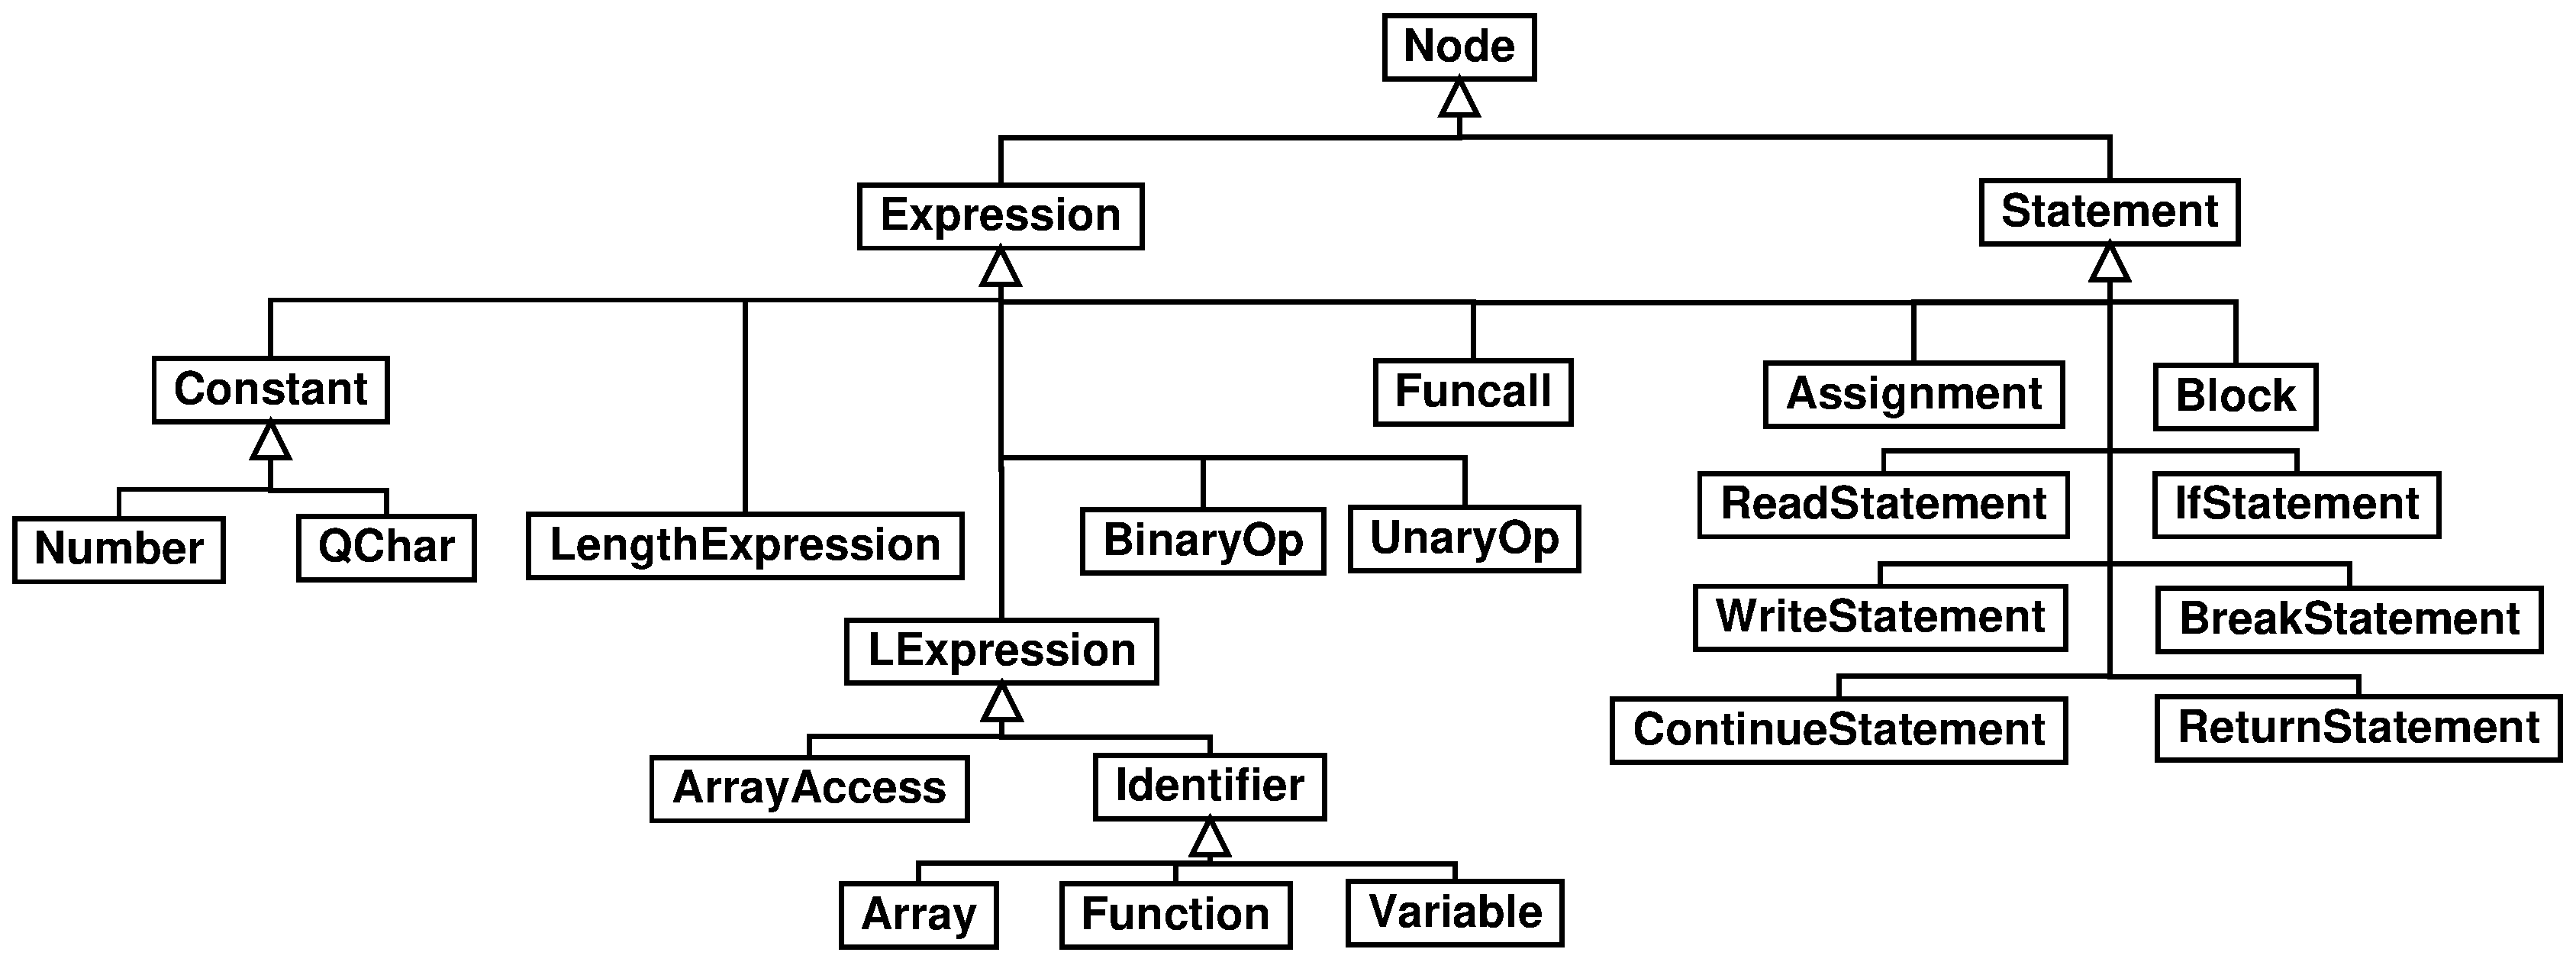
\includegraphics[width=1\textwidth]{syntaxtree_uml}
\caption{\label{syntaxtreediagram} The Abstract Syntax Tree Nodes}
\end{figure}
\end{center}

%%%%%%%%%%%%%%%%%%%%%%
\section{Code verification}
%%%%%%%%%%%%%%%%%%%%%%

This part of the compilation process will use visitors to traverse the syntax
tree constructed by the parser.

\subsection{Typechecking}

In a first step, the compiler will perform a static typecheck. This is
accomplished using the \texttt{TypeChecker} class, which is a subclass of a
\texttt{TreeVisitor}, and can thus traverse the syntax tree.

Whenever an error is encountered in the source text, the TypeChecker will
construct an error object, and append it to a list of errors. This errorlist
is the result of the typechecking process. If it is empty, no errors occured,
otherwise, all errors are printed (nicely formatted, with a reference to the
line number on which they occured) and the compilation process is aborted.

As an illustration, let us review a number of typecheck functions.

\paragraph{Typechecking if statements\\}

\begin{verbatim}
void TypeCheckVisitor::visitIfStatement(IfStatement* ifstmt) {
   ifstmt->condition()->accept(this);
   ifstmt->truebranch()->accept(this);
   ifstmt->falsebranch()->accept(this);

   Expression* condition = ifstmt->condition();
   if (!coerces_to(condition->type(),int_t)) {
      errors_->push_back(
        new ConditionError(condition->type(),
	                   condition));
   }
}
\end{verbatim}

First, the typechecker checks the condition and both branches of the if
statement. This is done through the ``double dispatch'' explained earlier.
When the typechecker has finished checking the branches, it checks to see
whether the expression is actually a conditional expression, i.e.~it's type
must be ``compatible'' with the primitive integer type (booleans are integers
in tiny). If this is not the case, the typechecker will append a
\texttt{ConditionError} to the errorlist.

\paragraph{Typecheking a Return statement\\}

\begin{verbatim}
void TypeCheckVisitor::visitReturnStatement(ReturnStatement* ret) {
   ret->expression()->accept(this);
   Type typeToReturn = ret->expression()->type();
   Type typeExpected = function_->returnType();
   if (!coerces_to(typeToReturn,typeExpected)) {
      errors_->push_back(
        new ReturnError(typeExpected,
	                typeToReturn, ret));
   }
}
\end{verbatim}

A Return Statement has one field, which is an expression to return. First, the
typechecker will check this expression. Afterwards, it asks for the type of
the expression (every expression has a type), and compares this with the
returntype of the function it is currently typechecking. If the types are not
compatble, the typechecker will append an appropriate error to the errorlist.

Other nodes are typechecked in a similar manner. When processing a
\texttt{Read} statement, for example, we must make sure we are not ``reading''
into an identifier denoting an array or a function. When processing a function
call, we must make sure the arity matches (ie.~that there are an equal number
of actual and formal arguments).

During the typechecking process, there will also be a check whether the
function with the signature \texttt{void tiny()} is well-defined. This
function is obligatory, since it is the ``main entry point'' of the program.

\subsection{Code analysis}

Code analysis is performed by the \texttt{LivenessChecker} visitor.
This visitor performs three checks:
\begin{itemize}
\item Check whether there are variables which are never used.
\item Check whether there are variables which are used before they might have
been initialized.
\item Check whether we reach the end of a non-void function.
\end{itemize}

This visitor will also traverse the abstract syntax tree to perform these
tasks. Let us illustrate the workings of the visitor by considering the
following example source code:
\begin{verbatim}
  {
    int x;
    int y;
    int z;
    y = ...
    if(...) {
      x = ...
      ...
    } else {
      ...
    }
    ...x... 
  }        
\end{verbatim}

\newcommand{\varset}[1]{
\textsl{\{#1\}}
}

Whenever the code analyzer processes a block, it will first scan all
declarations in the block and add them to a \texttt{VariableSet} (a simple
wrapper class around a set of variables). Thus, when starting, the variableset
is \varset{x,y,z}. When the analyzer next processes the assignment to $y$, it
will remove $y$ from the set of ``uninitialized'' variables, which is then
down to \varset{x,z}.

Whenever the analyzer processes a variable in an expression or statement, it
will just lookup the variable in the ``uninitialized'' set. If this variable
is found, this means a variable is used before it might have been initialized
(more about the ``might'' part later). If the variable was not found, this is
correct and the analyzer proceeds.

When checking an if-statement, we must be a little more careful: when visiting
the then-branch of an if-statement, we might encounter an assignment to
$x$, thus, the set is down to \varset{z}. However, imagine (as in the
example), that the else-branch does not ``define'' $x$. This means that, after
processing the if-statement, the set must remain \varset{x,z}. This is solved
as follows.

When processing an if-statement, the variableset is duplicated, thus we have
two sets: $\varset{x,z}_{then}$ and $\varset{x,z}_{else}$. When processing the
definition of $x$, we get $\varset{z}_{then}$ but the other set remains
unchanged. After processing the if statement, we just take the union of both
sets, i.e.~ $\varset{z}_{then} \cup \varset{x,z}_{else} = \varset{x,z}$.
If $x$ is thus subsequently used after the if, it still \emph{might} not have
been initialized.

A similar reasoning is applied for a while-statement: the condition of a while
might immediately fail, thus, there is a chance that the body of the while
statement will never be executed. Therefore, after visiting the while body,
just discard that variableset and continue using the variableset we had before
we started visiting the while, because no assignment in the while body can be
of importance afterwards (for this visitor).

When processing a \texttt{read} statement, we also remove the variable that is
read to from the ``uninitialized set. Thus, for this checker,
\texttt{y = \ldots{}} is equivalent to \texttt{read y}.

Apart from the ``uninitialized'' set, we also keep track of all ``used''
variables, in a similar manner. We start out with \varset{x,y,z}, remove $y$
when assiging to it, and also remove $x$ when using it. In the end, the set
will be down to \varset{z}. This means $z$ was never encountered, but it was
declared. $z$ is an unused variable. At the end of the process, raise an error
for each variable still in the ``unused'' set.

We now know how the analyzer finds uninitialized and unused variables. What
about checking whether we can reach the end of a non-void function? This
appears to be extremely easy. When starting to check a function whose return
type is non-void, insert a ``dummy'' $RETURN$ variable. Thus, in our example,
the variable set starts out as \varset{x,y,z,$RETURN$}.

Whenever we are then processing a \texttt{return} instruction, we will just
remove the dummy $RETURN$ variable from the set of ``uninitialized''
variables. All we have to do now is checking, after we have analyzed the
function body, whether the $RETURN$ variable is still in the set. If it is,
then this means there is a path in the code which can lead to the end of the
function without having performed a return.

Note that, when visiting an if or while statement, we have to ``save'' our
previous variablesets, because if and while statements may be arbitrarily
nested! This is taken care of by saving the variablesets on the runtime stack
before visiting the branches of an if or the body of a while statement.

\subsection{Constant folding}

Constant folding is done by the \texttt{ConstantFolder} treevisitor.  
The folder traverses the syntax tree and will examine each node. When a node
can be folded, it will be replaced by a semantically equivalent node. An
archetypical example of constant folding is an expression like \texttt{x=2+3},
which is transformed to an assignment node, containing a reference to $x$, and
a binary expression on the right hand side. This binary expression itself has
as its children $2$ and $3$, both wrapped in a \texttt{Number} node class.

The goal of the constantfolder, then, is to replace such a tree, consisting of
three nodes, by one node, namely a \texttt{Number} representing $5$. The
constant folder checks a binary operation as follows: first, visit (and
possibly fold) both arguments of the binary operation. Next, check whether
both arguments are constants (i.e.~numbers or characters). If this is the
case, we can perform a compile-time computation, and replace the binary
operation by the result of this computation.

To support this compile-time computation, and to easily allow new operations
in the source language, all operators are also represented as classes. Thus,
there is a \texttt{Plus} class, a \texttt{Divides} class, etc\ldots{}

The constant folder can then ask the operator to compute its result given both
arguments. If we decide to add a new operator to the tiny language, we only
have to subclass the \texttt{Operator} class, fill in its interface, and the
constantfolder will immediately be able to fold the new operator. This proves
the extendability you get when working with objects.

As a small ``extra'', the constantfolder will also check whether the
conditional expression of an if or while statement is a constant, if it is, it
will evaluate the if or while. For example, if we know at compile time
the if-condition evaluates to true, just replace the if with the then-branch.
These foldings are of course rather unnecessary, who would write an
if-statement if the result of the test is already known?

%%%%%%%%%%%%%%%%%%%%%%
\section{Intermediate code generation}
%%%%%%%%%%%%%%%%%%%%%%

Tiny generates a special form of intermediate code generally known as ``three
address code'' because an instruction constains at most three operand
``addresses''.

\subsection{Instruction overview}

This section describes all possible three-address instructions generated
by the compiler. In what follows, $a$ is assumed to be an array, $x$, $y$ and
$z$ can be variables or constants and $f$ represents a function.

It is important to note that instructions take as arguments not the abstract
syntax tree nodes \texttt{Variable}, \texttt{Array}, \texttt{Number},
etc\ldots{}, but their instruction counterparts: \texttt{VarRegister},
\texttt{ArrayRegister}, \texttt{NumRegister}, \ldots{}. This clearly decouples
the instruction code from the abstract syntaxtree, which is now no longer
needed.

\newcommand{\instr}[1]{
  \begin{center}
    \begin{tabular}{|c|}
    \hline
    \textbf{\texttt{#1}}\\
    \hline
  \end{tabular}
\end{center}
}

\paragraph{Array Access\\}
\instr{x = a[y]}

An instruction representing the accessing of an array. $y$ must be an integer
constant or variable. $x$ is a variable with as type the base type of the
array. Note that $x$ can also be a ``temporary'' variable. Temporaries can be
declared using the symboltable. The symboltable will ensure the declared
temporary is unique. Temporaries are given a number as a name, to print out a
temporary, a ``t'' is prepended, thus, the first temporary generated is
\texttt{t0} (unless \texttt{t0} is a ``real'' variable of course).

A second, important note about these instructions is that multi-dimensional
arrays in tiny are represented as \textbf{one-dimensional} arrays in the
intermediate (and generated) code! This means that statements of the form
\texttt{x = a[2][3]} will have to be translated to a one-dimensional access of
the form \texttt{x = a[offset*2+3]}.

Thus, if $t4$ would contain the value of $offset*2+3$, then one could generate
the instruction \texttt{t5 = a[t4]}. Usually, the target of this instruction
will be a temporary, this will generate redundancies, which are removed during
optimization.

\paragraph{Array Assignment\\}
\instr{a[x] = y}

An instruction representing assignment into an array. Here, $x$ is also a
``folded'' index in the case of a multi-dimensional array.

\paragraph{Array Allocation\\}
\instr{a = ARRAY x,y}

Creates a new array of length $x$, with $y$ dimensions. Store the result in
$a$. Note that $x$ denotes the length of a one-dimensional array.
For example, the array declared as \texttt{int[2][3] a}, gives rise to the
following code:
\begin{center}
\texttt{t0 = 1}\\
\texttt{t0 = t0 * 2}\\
\texttt{t0 = t0 * 3}\\
\texttt{a = ARRAY t0,2}\\
\end{center}

First, code is generated for the one-dimensional length of the
multi-dimensional array, which is $length_{dimension_1} \cdot \ldots \cdot
length_{dimension_n}$. Next, space for $a$ is allocated. If the dimension
is larger than one, extra code for handling the dimensions will have to be
generated.

\paragraph{Array Parameter\\}
\instr{ARRAYPARAM a}

Passes an array by reference to a function. The instruction requires just a
reference to the array to pass.

\paragraph{Simple Assignment\\}
\instr{x = y}

Simply assigns the value of $y$ to $x$.

\paragraph{Binary Operation\\}
\instr{x = y \textsl{op} z}

The binary operation instruction takes two argument registers, a target
register, and an operator $op \in$ \varset{$+$,$-$,$\times$,$\div$}.

\paragraph{Function Call\\}
\instr{CALL f,x}

Calls the given function, with as arguments the arguments loaded ``on top of
stack'' by the \texttt{PARAM} instructions. The number of arguments are also
passed to the instruction.

\paragraph{Dimension Length\\}
\instr{x = DIMLENGTH a,y}

Stores the length of dimension $y$ of the multi-dimensional array $a$ in $x$.
These instructions are necessary to retrieve the length of only one specific
dimension of a multi-dimensional array.

The \texttt{LENGTH} instruction only returns the \textbf{entire} length of
the array. Since multidimensional arrays are represented as one-dimensional arrays,
the length of such a multidimensional array is actually the product of all its
dimension lengths. However, we need the length of a dimension to calculate
offsets for \textsl{Array Assignment} and \textsl{Array Access} instructions.
Thus, the target of this instruction represents the mysterious $offset$
variable in the description of the \textsl{Array Access}.

\paragraph{Unconditional jump\\}
\instr{GOTO label}

A \texttt{GOTO} instruction jumps to the specified label. Labels are represented by
integers. Three address code is ``indexed'' code. A series of three address
instructions is represented as an instance of the class \texttt{Instructions}.
This class also provides some operators that come in handly, like
\texttt{operator[](Label)}. Thus, a \texttt{GOTO} instruction's destination
instruction can be retrieved by indexing the instruction ``stream'':\\
\texttt{Instruction destination = instructions[goto.label];}

\paragraph{Conditional jump\\}
\instr{IF x \textsl{op} y GOTO label}

This instruction only jumps to the destination if the test succeeds,
otherwise, the next instruction is executed. $op \in$ \varset{$<$,$>$,$=$,$\neq$}.

\paragraph{Array Length\\}
\instr{x = LENGTH a}

Retrieves the length of $a$ and stores it in $x$. Note that this returns the
one-dimensional length of $a$, not the length of any of its dimensions (use
\texttt{DIMLENGTH} instructions for that).

\paragraph{Multidimensional array declaration\\}
\instr{MULTIARRAY a}

Declares $a$ to be a multi-dimensional array. This instruction will call upon the
runtime environment (section \ref{runtime}) to use the \texttt{MULTIDIM} (see
below) instructions to store the dimension lengths of $a$. Afterwards, they
can be retrieved by \texttt{DIMLENGTH} instructions. 

\paragraph{Multidimensional length declaration\\}
\instr{MULTIDIM a,x,y}

Declares that dimension $x$ of array $a$ has length $y$.
For example, when declaring an array (in the source code) as \texttt{int[2][3] a},
this will give rise to the following instructions:
\begin{center}
\texttt{MULTIDIM a,0,2}\\
\texttt{MULTIDIM a,1,3}\\
\end{center}

The reason why these instructions were added to the instructionset will become
clear in section \ref{runtime}. For one-dimensional arrays, there is no
\texttt{MULTIDIM} instruction generated.

\paragraph{Parameter\\}
\instr{PARAM x}

Conceptually pushes $x$ onto the stack to pass it as a parameter to the
function called by the next \texttt{CALL} instruction. This instruction cannot
be used for passing arrays.

\paragraph{Reading input\\}
\instr{READ x}

Reads from standard input and stores the result in $x$. The read value is
converted to an integer or character appropriately. $x$ cannot be an array,
statements like \texttt{read a[x]} are transformed to:
\begin{center}
\texttt{READ t0}\\
\texttt{a[x] = t0}\\
\end{center}

\paragraph{Return\\}
\instr{RETURN x}

Returns from the function immediately and passes $x$ as the return value to
the caller.

\paragraph{Return Value\\}
\instr{RETVAL x}

This instruction is used to retrieve the return value from the callee. It is a
separate instruction because some function calls do not return a value, and some
functions can be called as a ``statement'' rather than as an expression. In
that case, there is no need to generate a \texttt{RETVAL} instruction.

\paragraph{Unary Assignment\\}
\instr{x = \textsl{unop} y}

Perform a unary operation on $y$ and store the result in $x$. Currently,
$unop$ can only be $-$.

\paragraph{Writing output\\}
\instr{WRITE x}

Writes the value of x to standard output. If $x$ denotes a character, the
character will be printed, otherwise, a number will be printed.

\subsection{Generating instructions}

Generating code from the abstract syntax tree is done using yet another
visitor: the \texttt{ICTranslator}. Most of this code generation is quite
straightforward and usually boils down to creating the right instruction and
appending it to the instructionstream.

Usually, temporary variables will have to be created to store results. This is
mostly the case with expressions. Expressions like \texttt{2+x/4*y} cannot
directly be translated using an instruction in the instructionset. Instead,
the expression must be translated to code like:
\begin{center}
\texttt{t0 = 2 + x}\\
\texttt{t1 = 4 * y}\\
\texttt{t2 = t0 / t1}\\
\end{center}

The result of the expression is generated in $t2$, and can then be further
used in another expression or statement. Like this, the entire syntaxtree is
traversed and converted to three address code.

\subsubsection{Backpatching goto's}

The trickiest part of generating three address code is the generation of if
and while statements. These statements cause the generation of \texttt{GOTO}
instructions. Sometimes, these \texttt{GOTO} instructions do not know where to
jump to yet, because the code where they jump to is not yet generated. The
following is part of the code which translates if-statements.

When the \texttt{ICTranslator} visits an If statement. It will first let a
\texttt{BExpTranslator} visit the If condition. A BExpTranslator is a
specialised code generator for boolean expressions. It will set up the code
for the boolean expression, including \texttt{GOTO}'s, but will leave their destination
blank.

\begin{verbatim}
void ICTranslator::visitIfStatement(IfStatement* ifstmt) {
  BexpTranslator bexpvisitor(this);

  //generate code for the boolean expression
  ifstmt->condition()->accept(&bexpvisitor);
\end{verbatim}

Just before the \texttt{ICTranslator} starts generating code for the
then-branche, it will save the label of the next instruction. After generating
the then-branche code, it will generate a \texttt{GOTO} which is meant to jump
over the else-branch. It's destination is at this point unknown.

\begin{verbatim}
  //the true exit for bexp should be rerouted to here
  Label trueExit = codestream_.nextInstructionLabel();
  ifstmt->truebranch()->accept(this);

  //generate an escape for stmt1 to jump over stmt2 when done
  GotoI* gotoEnd = new GotoI(0);
  codestream_ << gotoEnd;
\end{verbatim}

Next, the translator generates code for the else-branch, saving the first
label of that branch first. After visiting the else-branch, the translator now
knows the address to which the ``escape'' \texttt{GOTO} should be rerouted.

\begin{verbatim}
  //the false exit of bexp should be rerouted to here
  Label falseExit = codestream_.nextInstructionLabel();
  ifstmt->falsebranch()->accept(this);

  //the escape goto should be rerouted to here
  Label endExit = codestream_.nextInstructionLabel();
  gotoEnd->setDestination(endExit);
\end{verbatim}

It remains to backpatch the \texttt{GOTO's} that the \texttt{BExpTranslator}
generated. This is done as follows: whenever the BExpTranslator generates a
\texttt{GOTO} with an unknown destination, it adds it to a set of
instructions. The instruction is added to the \texttt{trueSet} if it is meant
to jump to the then-branch, and added to the \texttt{falseSet} if it is meant
to jump to the else-branch.

All the translator has to do is to set the destination of all instructions in
the \texttt{trueSet} to the saved label of the then-branch, and the
destination of all instructions in the \texttt{falseSet} to the saved label of
the else-branch. A similar reasoning is applied to generate code for the
condition of a while statement: the \texttt{trueSet} instructions jump to the while
body, the \texttt{falseSet} instructions jump over the while.

\begin{verbatim}
  //backpatch the boolean expression
  backpatch(bexpvisitor.trueSet(),codestream_,trueExit);
  backpatch(bexpvisitor.falseSet(),codestream_,falseExit);
}
\end{verbatim}

The tiny compiler also adds two new statements to the tiny specification: a
\texttt{break} and a \texttt{continue} statement. These statements can only be used in the body of a while (or for) loop. A \texttt{break} is translated to a \texttt{GOTO} to the instruction following the while. A \texttt{continue} statement is translated to a \texttt{GOTO} to the beginning of the evaluation of the while condition.

A final note on the BExpTranslator: this translator will translate the
logical NOT (\texttt{!}) merely by switching the true and false sets. A
similar reasoning can be applied for logical AND and OR, but these are not
implemented. Note that a BexpTranslator will translate, for example, $x < y$ as\\
\texttt{IF x < y GOTO true exit}\\
\texttt{GOTO false exit}\\

An \texttt{ICTranslator} will translate $x < y$ as\\
\texttt{1. IF x < y GOTO 4}\\
\texttt{2. t0 = 0}\\
\texttt{3. GOTO 5}\\
\texttt{4. t0 = 1}\\

In other words: a \texttt{BExpTranslator} translates boolean expressions
\textsl{by flow of control}, while an \texttt{ICTranslator} translates boolean
expressions \textsl{by value}. The translation by value is necessary when
evaluating code like \texttt{x = (y < z)}. In that case, we want a boolean
value stored in x. In the case of \texttt{if (y < z) \ldots{}} it would be
stupid to evaluate $y<z$ by value, and then jumping according to the test
$t0 \neq 0$.

%%%%%%%%%%%%%%%%%%%%%%
\section{Code optimization}
%%%%%%%%%%%%%%%%%%%%%%

When the \texttt{ICTranslator} has generated the code, there are usually lots
of redundant temporary variables generated. Moreover, it might be the case
that code for the same expression is generated multiple times.

The optimization algorithm is designed to remove these redundancies. The
algorithm will first partition the generated code into so called ``basic
blocks''. Each basic block is then transformed into a DAG which allows local
``common subexpression elimination''.

\subsection{Basic Blocks}

A basic block is a piece of code that has to be executed in its entirety
(i.e.~it cannot contain \texttt{GOTO}'s that exit the block somewhere in the
middle, if there is a \texttt{GOTO} instruction, it must be last). No
instruction except for the first can be the target of a goto instruction
(otherwise it could also be that only part of the block is executed).

Basic blocks can be easily identified by marking the targets of goto's and
instructions after goto's. These ``marked'' instructions identify the
beginning of a basic block and are called ``leaders''.

A basic block is represented by the compiler as a vector of \texttt{Instruction}s.
Before the optimization algorithm is applied, the generated intermediate code
for a function body is partitioned into these basic blocks.

Each basic block is then fed to the optimization algorithm. Usually,
an optimized block will contain less instructions, which means the labels of
the instructions have changed. Therefore, when each basic block is optimized,
the labels are ``relocated'' so that the destination of a \texttt{GOTO} before
optimization is adapted to the new location.

Since destination instructions of \texttt{GOTO}s are by definition leaders,
it suffices to associate the old and new labels (through a mapping) of the
leaders, to be able to relocate the \texttt{GOTO} labels.

\subsection{DAG optimization}

The DAG optimization is performed by two large visitor classes:
\texttt{BB2DagMapper} and \texttt{Optimizer}.

The \texttt{BB2DagMapper} takes a basic block as input, and will transform
this block to a DAG or \textsl{directed acyclic graph}. The goal here is to
remove redundant computations (i.e.~calculating something whose value is
already calculated in another register), and to reduce the number of temporary
registers.

\subsubsection{Optimizing binary operations}

To see how this mapping from code to a graph is done, let us examine the case
of a binary operation: \texttt{x = y + z}, for example. The mapper will visit
each three address code instruction, and map it to a series of nodes.

First, the mapper will check whether there already exists a node for $y$ and
$z$. A lookup is performed and a node is returned. This returned node might be
a nullpointer, or it might be that the node was ``killed'' by another
instruction. In that case, \texttt{isValid} returns false, and a new leaf is
made. Leafs contain the register they represent.

\begin{verbatim}
void BB2DagMapper::visitBinaryAssInstruction(BinAssignmentI* bas) {
  //retrieve both child nodes (or create new ones)
  DagNode* ynode = lookupNode(bas->getFirstArg());
  if (!isValid(ynode))
    ynode = makeLeaf(bas->getFirstArg());
  DagNode* znode = lookupNode(bas->getSecondArg());
  if (!isValid(znode))
    znode = makeLeaf(bas->getSecondArg());
\end{verbatim}

The mapper now has two child nodes for $y$ and $z$, either previously created
or newly made. Note that a \texttt{DagLeaf} is a subclass of \texttt{DagNode},
so we do not know (or care) if the nodes found are really nodes or leaves.

Next, we have to create a node which represents the \texttt{y+z} code.
We do this by first searching the DAG for an already existing \texttt{y+z}
node. The match algorithm also handles algebra\"ic identities and
commutativity for operators, thus it would match the node \texttt{z+y} if it
existed.

If no match is found, we have to insert a new node into the DAG. Every
\texttt{DagNode} has three children (note that a three-address instruction can
contain at most three operands), but this node will require only two children
($y$ and $z$), thus the third child is null.

\begin{verbatim}
  //look for an already existing 'y op z' node (with algebraic matching)
  DagNode* existingNode = match(*bas->getOperator(),ynode,znode);
  if (!isValid(existingNode)) {
    string opcode(bas->getOperator()->symbol());
    existingNode = makeNode(bas,ynode,znode,0);
    addToDAG(opcode,existingNode);
  }
\end{verbatim}

If a match is found, we already have an \texttt{y+z} node in the DAG. This is
the basis of the ``common subexpression elimination'': instead of adding a new
node, we just add $x$ as a ``target'' of the existing node. When the optimized
code is generated, it will calculate the value of $y+z$ only once, and assign
the result to each of its ``targets''. 

\begin{verbatim}
  (*nodes_)[bas->getTarget()] = existingNode;
  addTarget(existingNode, bas->getTarget());
}
\end{verbatim}

We also keep a mapping from variable(registers) to nodes. The \texttt{nodes\_}
mapping returns, for a given variable, the node containing the current
``value'' for that variable. Since, we just assigned a value to $x$ (namely
$y+z$), we should set the current ``valuenode'' of $x$ to the \texttt{y+z}
node.

\subsubsection{Peculiarities}

There are a number of cases in which translating code to a DAG is not so
straightforward. These cases are caught by the DAG algorithm. A brief
overview:

\begin{itemize}
\item Sometimes, a variable's ``value'' is used by another node (i.e.~the node
is dependent on that variable), but there is another node which assigns to
that variable. In that case, optimized code must be arranged to generate code
for the depending node \textbf{first}, before generating the code which causes
the assignment.

The DAG algorithm solves this by adding extra edges from nodes to other
nodes which represent the ``value'' of the variable the node depends on.
The importance of these edges will be discussed when mapping the DAG back to
code (see section \ref{optimizingcode}).

\item When processing \textsl{Array Assignment} instructions, one has to be
careful to not rearrange the code in arbitrary ways. A simple example
illustrates the case:\\
\begin{center}
\texttt{x = a[y]}\\
\texttt{a[u] = v}\\
\texttt{z = a[y]}\\
\end{center}

A naive common subexpression elimination algorithm would translate this to\\
\begin{center}
\texttt{x = a[y]}\\
\texttt{z = x}\\
\texttt{a[u] = v}\\
\end{center}

which may be incorrect! $z$ is different from $x$ if $u = y$ and $v \neq x$.
The solution here is to have the \textsl{Array Assignment} instruction
\texttt{a[u] = v} \textbf{kill} all nodes in the DAG so far, representing
\textsl{Array Access} instructions accesing $a$.
In this way, $z$ will get its own \textsl{Array Access} node,
and there will be no sharing with $x$'s node.

Even with this sharing removed, we must remain careful. The following code is
also incorrect:\\
\begin{center}
\texttt{x = a[y]}\\
\texttt{z = a[y]}\\
\texttt{a[u] = v}\\
\end{center}

It is clear that the \texttt{z = a[y]} instruction must be generated
\emph{after} the array assignment, while the \texttt{x = a[y]} instruction
must be generated \emph{before} it. This is solved in a similar manner as the
case outlined above, by adding extra ``edges'' between the nodes.

\item Another, very similar problem arises with function calls. Imagine the
following code:\\
\begin{center}
\texttt{x = y + z}\\
\texttt{CALL f}\\
\texttt{u = y + z}\\
\end{center}

Clearly, we can perform common subexpression elimination and remove one
redundant addition. This is also what the algorithm does, provided however,
that all these variables are \emph{local} variables. If any of them are global
however, then we cannot just perform the common subexpression elimination. If
$x$ would be global, and $f$ modifies $x$, then we cannot just add \texttt{u = x}.

This is handled similarly by having a \texttt{CALL} instruction kill every
node in the DAG which depends upon, or modifies a global variable. Just as
with arrays, we also cannot arbitrarily change the order of the statements in
this block: $f$ might use $u$ for example, so we cannot generate the
assignment to $u$ until after the \texttt{CALL}. This is, again, solved
through extra ``edges'' in the DAG.
\end{itemize}

\subsubsection{Generating the optimized code}
\label{optimizingcode}

Generating the code is a matter of mapping the constructed DAG back to three
address code (to a basic block). This is done by a very simple algorithm,
which uses the edges between the nodes to create an ordening between the code
fragments.

In the previous paragraph, it was explained, that to ``force'' the generation
of some node's code before some other node's code, it suffices to add a
``constraining'' edge between them. Next to its maximum of three operand
children, a node also contains a number of edges to nodes whose code needs to
be generated before the orignating node's code.

The code generating algorithm now works as follows: starting from the
``greatest'' elements in the DAG (these are the nodes without a parent, and
thus the nodes which are ``highest'' in the DAG), generate code for the
children and referred nodes first. This is done by a recursive algorithm which
will first generate code for the references:

\begin{verbatim}
void BB2DagMapper::optimizeNode(DagNode* node) {
  //if code for the node is already generated, return
  if (node->generated())
    return;
  //generate code for the references first
  DagNodes* refs = node->references();
  for (DagNodes::iterator ref = refs->begin();
                          ref!=refs->end(); ref++) {
    optimizeNode(*ref);
  }
\end{verbatim}

Note that a node contains a boolean denoting whether or not code for the node
has already been generated. If a node's code is already generated, we
immediately return from the call. This is necessary since a node can be
referred to by more than one node (a node can have more than one parent,
that's why it's a graph and not a tree).

Next, we still need to generate code for the children, which is evident
because the children should be ``initialized'' before they can be used by
another instruction. A check is necessary since a child can be a nullpointer
(some nodes have less than three children).

\begin{verbatim}
  //generate code for the children
  if (node->firstChild())
    optimizeNode(node->firstChild());
  if (node->secondChild())
    optimizeNode(node->secondChild());
  if (node->thirdChild())
    optimizeNode(node->thirdChild());
  node->setGenerated();
  optimizer_->accept(node);
}
\end{verbatim}

When code for the children is generated, all we need to do is generate code
for the current node itself, and to mark that node's code as being generated.
Optimizing the code is done by another visitor, the \texttt{Optimizer}. An
optimizer will examine the original instruction, and create a new instruction
which usually takes new operands.

Imagine the unoptimized code being as follows:\\
\begin{center}
\texttt{t0 = x + y}\\
\texttt{z = t0 + 3}\\
\texttt{t1 = x + y}\\
\texttt{u = t1 * 2}\\
\end{center}

It is clear that \texttt{x + y} is a common subexpression which can be
eliminated. We could for example just ignore the third instruction, but then
we must make sure that $t1$ is ``replaced'' by $t0$ in the fourth instruction:\\
\begin{center}
\texttt{t0 = x + y}\\
\texttt{z = t0 + 3}\\
\texttt{u = t0 * 2}\\
\end{center}

This is taken care of by the optimizer. Another important function of the
optimizer is to decrease the number of used temporary registers. A common
pattern of generated code is:
\begin{center}
\texttt{t0 = a[x]}\\
\texttt{y = t0}\\
\end{center}

This kind of code is typical for the generated code of expressions, where
parts of the expression's value are stored in temporaries. The optimizer will
notice the redundancy and transform this code to:\\
\begin{center}
\texttt{y = a[x]}\\
\end{center}

%%%%%%%%%%%%%%%%%%%%%%
\section{Code generation}
%%%%%%%%%%%%%%%%%%%%%%

The ``back end'' of the compiler consists of transforming the optimized three
address code to the target language. In this case, this is JVM assembler, more
specifically a dialect of the language, suitable for processing by
\texttt{javaa}.

The generated JVM syntax is quite straightforward when it comes to method
declaration and instruction generation. The code is still quite readable.
The greatest difference between the three address code and the JVM assembler
code is that three address code works with assignment instructions operating
on ``virtual registers'', whereas JVM instructions usually operate on operands
on top of the runtime stack.

\subsection{Generated JVM Class Layout}

Tiny generates a JVM assembler source text which has the
following layout (in Java syntax):
\begin{verbatim}
    //basename is the name passed in through the command-line
    public class basename {

       public static int a_global;

       public static int[] a_global_array;

       public static void main(String[] args) {
          //code for initialization of globals,
          //code which allocates space for a_global_array
          //comes here

          //call 'void tiny()'
          invokestatic void tiny()
          return
       }

       public static void tiny() {
          //code for tiny
       }

       public static int a_function(int[] a) {
          //code for a_function, local variables
          //are also declared locally here
       }
    }
\end{verbatim}

What is important is that each global variable is modelled as a static class
variable, and each function is modelled as a static (class) method. These methods
do not require an object to be passed when it is called.

Initialization code for globals is executed in the \texttt{main} function, and
is thus always executed first, before the tiny program runs. The tiny program
itself is then started by a call to the \texttt{tiny} function, which is
obligatory for each tiny program. From then on, the tiny program can call
other implemented tiny functions, and it can use local variables, which are
also declared as local variables in the JVM assembler.

Since assembler does not know the concept of ``blocks'' or scopes, we need to
solve the problem that multiple variables with the same name may be declared
in different scopes, for example:\\
\begin{verbatim}
    void f() {
      int x;
      { int x;
        ...
      }
      ...
    }
\end{verbatim}

This is done by adjusting the name of identifiers according to their scope
level. The outer $x$ is renamed to \texttt{f\_x}, the inner $x$ to
\texttt{f\_block\_x}. In the JVM assembler, the code can then work with
both variables in the same scope:
\begin{verbatim}
    int f_x;
    int f_block_x;
    ...
\end{verbatim}

\subsection{JVM Code generation}

This section explains how each intermediate code instruction is translated to
JVM assembler instructions.

\newcommand{\translate}[2]{
\instr{#1}
\begin{center}
$\downarrow$
\end{center}
\begin{center}
\begin{tabular}{|l|}
\hline
#2\\
\hline
\end{tabular}
\end{center}
}


\paragraph{Array Access\\}
\translate
{x = a[y]}
{
aload a\\
load y\\
iaload\\
store x
}

\paragraph{Array Assignment\\}
\translate
{a[x] = y}
{
aload a\\
load x\\
load y\\
iastore
}

\paragraph{Array Allocation\\}
\translate
{a = ARRAY x,y}
{
load x\\
newarray a.basetype\\
store a\\
int\texttt{[]} \_a\_dimensions\_\\
ldc y\\
newarray int\\
astore \_a\_dimensions\_
}

For one-dimensional arrays, the last four statements are not generated. These
statements are needed when declaring multi-dimensional arrays. Their purpose
will be explained in section \ref{runtime}.

\paragraph{Array Parameter\\}
\translate
{ARRAYPARAM a}
{aload a}

In Java, parameters are passed by just pushing them on the stack. A function
requiring $n$ arguments will use the $n$ topmost arguments on the runtime
stack.

\paragraph{Simple Assignment\\}
\translate
{x = y}
{
load y\\
store x
}

It must be noted that integers and characters are actually loaded using the
\texttt{iload} command. However, the \texttt{load} command is also allowed,
and \texttt{javaa} would also transform this to an \texttt{iload} command
automatically.

\paragraph{Binary Operation\\}
\translate
{x = y \textsl{op} z}
{
load y\\
load z\\
opcode(op)\\
store x
}

The opcode depends, of course, on the kind of operator. The table below lists
the opcodes of each binary operator:
\begin{center}
\begin{tabular}{|c|c|}
\hline
Operator & Opcode \\
\hline
$+$ & \texttt{iadd} \\
$-$ & \texttt{isub} \\
$\times$ & \texttt{imul} \\
$\div$ & \texttt{idiv} \\
\hline
\end{tabular}
\end{center}

\paragraph{Function Call\\}
\translate
{CALL f,x}
{invokestatic f.returntype f(f.argtypes)}

Since every tiny function is modeled as a static member function, just use the
\texttt{invokestatic} command. Arguments are taken from the top of stack.

\paragraph{Dimension Length\\}
\translate
{x = DIMLENGTH a,y}
{
aload a\\
ldc y\\
invokestatic int TinyRuntime.dimension(Object,int)\\
istore x
}

To retrieve the length of a specific dimension, a call is made to a runtime
function which returns just this dimension length. The returned length is
stored in $x$.

\paragraph{Unconditional jump\\}
\translate
{GOTO label}
{goto label}

\texttt{GOTO}'s are conveniently mapped to JVM goto's. The most important part
is, of course, the representation of the labels. Remember that three address
code was indexed code, and labels were represented as indices into this code
sequence.

These indices are translated to JVM labels in a very straightforward way:
label $n$ is represented as the string $Ln$ in JVM syntax. Labels are only generated in
front of ``leader'' instructions, since these are the only instructions that
can be jumped to.

\paragraph{Conditional jump\\}
\translate
{IF x \textsl{op} y GOTO label}
{
load x\\
load y\\
opcode(op)
}

Again, the opcode depends on the type of relational operator. The
possibilities are listed below:
\begin{center}
\begin{tabular}{|c|c|}
\hline
Operator & Opcode \\
\hline
$<$ & \texttt{if\_icmplt} \\
$>$ & \texttt{if\_icmpgt} \\
$=$ & \texttt{if\_icmpeq} \\
$\neq$ & \texttt{if\_icmpne} \\
\hline
\end{tabular}
\end{center}

\paragraph{Array Length\\}
\translate
{x = LENGTH a}
{
aload a\\
arraylength\\
store x
}

\texttt{arraylength} retrieves the length of a Java array. Since all tiny
arrays (including multi-dimensional arrays) are modeled by one-dimensional
Java arrays, this length returns the product of the dimension lengths for
multi-dimensional arrays.

\paragraph{Multidimensional array declaration\\}
\translate
{MULTIARRAY a}
{
aload a\\
aload \_a\_dimensions\_\\
invokestatic void TinyRuntime.declareArray(Object,int\texttt{[]})
}

This instruction calls upon a runtime function to store the dimension lengths
(themselves stored in an array of integers) so that they can be retrieved by
\texttt{DIMLENGTH} instructions.

\paragraph{Multidimensional length declaration\\}
\translate
{MULTIDIM a,x,y}
{
aload \_a\_dimensions\_\\
ldc x\\
iload y\\
iastore
}

Sets the $x$'th dimension of array $a$ to $y$. This can be interpreted as an
instruction equivalent to \texttt{\_a\_dimensions\_[x] = y}.

\paragraph{Parameter\\}
\translate
{PARAM x}
{load x}

Just as with \texttt{ARRAYPARAM} instructions, the argument is just loaded on
top of stack.

\paragraph{Reading input\\}
\translate
{READ x}
{
getstatic java.io.InputStream java.lang.System.in\\
invokevirtual int java.io.InputStream.read()\\
i2c\\
invokestatic int java.lang.Character.getNumericValue(char)\\
store x
}

Reads a character read from standard input into $x$. This is done using the
Java standard input object \texttt{System.in} and the \texttt{InputStream.read} method. When reading into an integer however, we need to convert the read character into an integer. This is done using the class method \texttt{Character.getNumericValue}.

When reading into a character, the fourth statement is, of course, not
generated. Note the use of \texttt{i2c} which means casting an \texttt{int} to
a \texttt{char}. \texttt{read} returns an integer, but this integer is
actually the representation of a character (ie an int between $0$ and $255$).

\paragraph{Return\\}
\translate
{RETURN x}
{
load x\\
ireturn
}

Java returns the integer or character currently on top of stack, so just push
the value to return on top of stack, then return from the function.

\paragraph{Return Value\\}
\translate
{RETVAL x}
{store x}

When a function returns, it leaves the value on top of the runtime stack. This
value can then be accessed by the caller. We just have to store this variable
in $x$ so that it can be used afterwards.

\paragraph{Unary Assignment\\}
\translate
{x = \textsl{unop} y}
{
load y\\
opcode(unop)\\
store x
}

The only operand currently passed to this kind of instruction is the unary
negation, represented by the JVM instruction \texttt{ineg}. The negated value
of $y$ is left on top of stack, and subsequently saved into $x$.

\paragraph{Writing output\\}
\translate
{WRITE x}
{
getstatic java.io.PrintStream java.lang.System.out\\
load x\\
invokevirtual void java.io.PrintStream.print(int)
}

Writing to standard output is done via the equivalent of the typical java
syntax \texttt{System.out.println(...)}. If the value written is a character,
then\\ \texttt{java.io.PrintStream.print(char)} is called instead.

\subsection{JVM Optimizations}

The following list gives an overview of all optimizations performed on the
target language. Some of these optimisations are better known as ``peephole
optimization'' because they check the code for a certain pattern and replace
it with a more efficient one.

\begin{description}
\item[Efficient use of the runtime stack]
Unquestionably the most important optimization is the efficient usage of the
runtime java stack. The reason why this is so important is that is can save us
\textbf{many} uses of temporary variables.

Imagine the code
\begin{center}
\texttt{t0 = x + y}\\
\texttt{u = t0 + z}\\
\end{center}

Which is the intermediate code counterpart of the tiny code \texttt{u = x + y
+ z}. We can translate this code fragment in two ways: optimized or
unoptimized (the tiny compiler uses the optimized version):
\begin{center}
\begin{tabular}{|l|l|}
\hline
Unoptimized & Optimized \\
\hline
\texttt{iload x}  & \texttt{iload x}\\
\texttt{iload y}  & \texttt{iload y}\\
\texttt{iadd}     & \texttt{iadd}\\
\texttt{istore t0}& \\
\texttt{iload t0} & \\
\texttt{iload z}  & \texttt{iload z}\\
\texttt{iadd}     & \texttt{iadd}\\
\texttt{istore u} & \texttt{istore u}\\
\hline
\end{tabular}
\end{center}

At first sight, this optimization might seem easy to perform. For some cases,
as in the example, this is true. There are, however, exceptions. If the
intermediate code is:
\begin{center}
\texttt{t0 = x + y}\\
\texttt{u = z + t0}\\
\end{center}

This requires us to do more checking, because now we no longer have the easily
matched code fragment\\
\texttt{istore t0}\\
\texttt{iload t0}\\
but the fragment\\
\texttt{istore t0}\\
\texttt{iload z}\\
\texttt{iload t0}\\

There is another culprit: because of common subexpression elimination, it
might very well be that the variable $t0$ is used somewhere else in the code
(further down below). In that case, it is important that we generate the
otherwise redundant save and load instructions, because otherwise $t0$ will be
uninitialized! The compiler also handles these cases.

The optimization goes further than this. It will also try to optimize array
access and assignment instructions. Take an array access statement for
example:
\begin{center}
\texttt{t1 = ...}\\
\texttt{a[t1] = x}
\end{center}

Where $t1$ is a temporary. To generate code for the array assignment
instruction, the \texttt{iastore} instruction expects the arguments to be
on the runtime stack in the following order:
\begin{center}
\begin{tabular}{|c|}
value \\
index \\
array \\
\hline
\end{tabular}
\end{center}

However, in our example, the index, $t0$ is already on top of stack, but it
should come ``between'' the array and the value.
Instead of storing $t1$ in a local variable and loading it in the
right order, the compiler will use \texttt{swap} instructions to swap the
contents of the top of stack until they are in the right place, in our
example, the following code would be generated ($t1$ is currently on top of
stack):\\
\texttt{aload a} //$a$ is now on TOS, followed by $t1$ \\
\texttt{swap} //swaps $a$ and $t1$, $t1$ now on top of stack \\
\texttt{iload x} //load the value \\
\texttt{iastore} //store $x$ in $a$ at position $t0$ \\

This saves us a \texttt{save t0} and \texttt{load t0} instruction.

\item[Specialised instructions for constants]
The Java virtual machine has specialised instructions for loading small
constants. These instructions are usually faster, and take up less space in
the generated bytecode. Loading an integer on top of stack is done as follows
by the tiny compiler:
\begin{center}
\begin{tabular}{|l|l|}
\hline
Value & Instruction \\
\hline
$-1$ & \texttt{iconst\_m1} \\
$0\leq n \leq 5$ & \texttt{iconst\_n} \\
$-128 \leq n \leq 127$ & \texttt{bipush n} \\
any other integer & \texttt{ldc n} \\
\hline
\end{tabular}
\end{center}
\item[Specialised increment instruction]
The compiler will efficiently generate code for instructions of the form
\texttt{x = x + C}, \texttt{x = x - C} and \texttt{x = C + x}, as long as
$-127 \leq C \leq 128$. The generated instruction is then \texttt{iinc x C},
or \texttt{iinc x -C}.

\item[Temporary variable declarations]
The compiler will not generate declarations for temporary variables which
are discarded using the runtime stack.

\end{description}

\subsection{Runtime environment}
\label{runtime}

The instructions \texttt{DIMLENGTH} and \texttt{MULTIARRAY} use the two static
methods:
\begin{center}
\begin{tabular}{l}
\texttt{void declareArray(Object array, int[] dimensions)}\\
\texttt{int dimension(Object array, int dim)}\\
\end{tabular}
\end{center}

These methods are static member functions of the class \texttt{TinyRuntime}.
The methods of this class provide runtime support for multi-dimensional
arrays. To see why this is necessary, behold the following tiny code:
\begin{verbatim}
    void tiny() {
      int[2][3] a;
      f(a)
    }

    void f(int[0][0] b) {
      int x;
      x = b[1][2];
    }
\end{verbatim}

Note the type signature of $f$: the function cannot possibly know the size of
the array passed as an argument, whether one-dimensional or not. For
one-dimensional arrays, this is not much of a problem, the
\texttt{length} operator can be used to retrieve the length of the array.

It was already explained that tiny represents multi-dimensional arrays as
one-dimensional arrays. Thus, $a$ is internally declared as the java array
\texttt{int[6] a}. This implies that any access into $a$ must also be
translated to a ``one-dimensional'' address. Thus, the array access in $f$ is
encoded as: \texttt{x = b[1 * 3 + 2]}, where $3$ is the second dimension of
the array.

The only problem here is: how is $f$ to know, \textbf{at compile time} what
the dimensions of its formal parameter are? It is impossible to figure this
out at compile time, yet we have to generate the offset code at compile time!

This is solved by generating, at the beginning of a function taking a
multi-dimensional array as a formal parameter, a \texttt{DIMLENGTH}
instruction. This instruction queries the runtime environment for the
dimension length (through a call to \texttt{dimension}),
which is then stored in a temporary, say $t1$. From then on,
any array access to the formal is relative to $t1$.

Of course, if \texttt{DIMLENGTH} can retrieve the length of a given dimension,
that information must first have been given to the runtime environment (we
cannot insert this at compile time, because arrays may have arbitrary length,
only determinable at runtime).

The \texttt{MULTIDIM} and \texttt{MULTIARRAY} instructions will allocate, at
runtime an array containing the dimension lengths of the newly allocated
multi-dimensional array. This array will then be stored in the runtime
environment (through a call to \texttt{declareArray}).

The TinyRuntime class itself is nothing more than a class containing a mapping
which maps an array to its dimension information.

\end{document}
